%--------------------------------------------------------------- %
\documentclass[SPC-MASTER.tex]{subfiles}
\begin{document}
	\Large

\section{Nelson Rules for Interpreting Control Charts}
{\Large
\begin{itemize}
\item The eight tests used in statistical process control were developed by Lloyd S. Nelson, a process control expert. They are
based on his determination that the identified patterns are very unlikely to occur in stable processes.

\item Thus
the existence of any of these patterns in an $\bar{X}$ chart indicates that the process may be unstable, and that one or
more assignable causes may exist. 

\item The table on the next page contains examples of test failure for each of the eight tests,
with a description for each graph as to what is required for the illustrated test failure.

\item In practice, tests 1,2 and 7 are considered the three most useful.
\end{itemize}
}
{
\Large
\subsection{Descriptions of Tests}
\begin{description}
\item[Test 1 - 3 sigma rule] Identifies points outside of the control limits\\
Test 1 identifies points that are more standard deviations from the center line. Test 1 is
universally recognized as necessary for detecting out-of-control situations. It has a
false alarm rate of only 0.27\%.

\item[Test 2] Identifies shifts in the means \\
Test 2 signals when 9 points in a row fall on the same side of the center line.  The use of Test 2
significantly increases the sensitivity of the chart to detect small shifts in the mean.

When test 1 and test 2 are used together, significantly fewer subgroups are needed
to detect a small shift in the mean than are needed when test 1 is used alone.
Therefore, adding test 2 helps to detect common out-of-control situations and
increases sensitivity enough to warrant a slight increase in the false alarm rate.
\end{description}
}
\newpage
\begin{figure}[h!]
  % 
  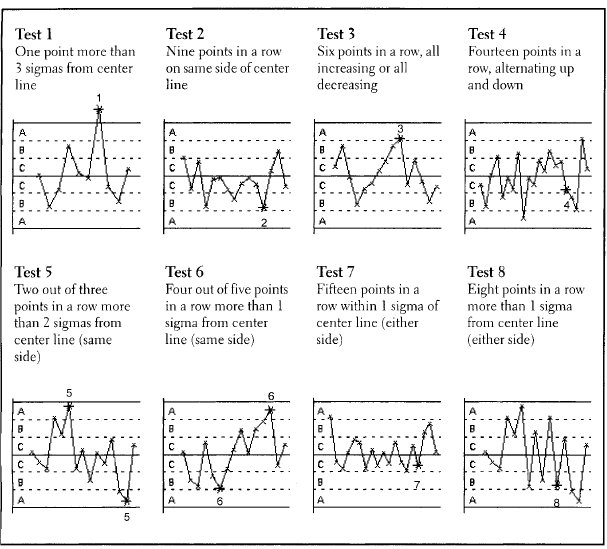
\includegraphics[scale=0.80]{WECOtests}\\
  %\caption{WECO Tests}\label{WECO}
\end{figure}

\newpage

\newpage
{
\large
\begin{description}
\item[Test 3] $k$ points in a row, all increasing or all decreasing\\
Test 3 is designed to detect drifts in the process mean.\\
However, when test 3 is used in addition to test 1 and test 2, it does not
significantly increase the sensitivity of the chart to detect drifts in the process
mean.


\item[Test 4] $k$ points in a row, alternating up and down\\
Although this pattern can occur in practice, it is recommended to search for any
unusual trends or patterns rather than test for one specific pattern.
\item[Test 5] $k$ out of k=1 points $> 2$ standard deviations from center line\\
This test is not quite as informative because it did not
uniquely identify special cause situations that are common in practice.
\item[Test 6] $k$ out of k+1 points $> 1$ standard deviation from the center line\\
This test is not quite as informative because it did not
uniquely identify special cause situations that are common in practice.

\item[Test 7] Identifies control limits that are too wide\\
Test 7 signals when 12 or 15 points in a row fall within 1 standard deviation of the
center line.\\ Test 7 is used only for the $\bar{X}$ chart when the control limits are
estimated from the data. When this test fails, the cause is usually a systemic source
of variation (stratification) within a subgroup, which is often the result of not 
forming rational subgroups. 
\item[Test 8] $k$ points in a row $> 1$ standard deviation from center line (either
side)\\
This test is not quite as informative because it did not
uniquely identify special cause situations that are common in practice.
\end{description}
}
\end{document}